\documentclass[11pt,a4paper]{article}

\usepackage[T1]{fontenc}
\usepackage[utf8]{inputenc}
\usepackage{lmodern}
\usepackage{geometry}
\usepackage{microtype}
\usepackage{amsmath,amssymb}
\usepackage{graphicx}
\usepackage{booktabs}
\usepackage{tabularx}
\usepackage{array}
\usepackage{enumitem}
\usepackage{float}
\usepackage{caption}
\usepackage{xcolor}
\usepackage{fancyhdr}
\usepackage{hyperref}

\geometry{top=22mm,bottom=23mm,left=23mm,right=23mm,headheight=15pt}
\graphicspath{{figures/}}

\definecolor{researchnavy}{HTML}{102A43}
\definecolor{researchblue}{HTML}{1D4ED8}
\definecolor{researchteal}{HTML}{0F766E}
\definecolor{researchgray}{HTML}{52606D}
\definecolor{researchlight}{HTML}{F4F7FA}
\definecolor{researchline}{HTML}{CBD5E1}

\hypersetup{
  colorlinks=true,
  linkcolor=researchblue,
  citecolor=researchteal,
  urlcolor=researchblue,
  pdftitle={Adversarial Robustness Across Verification and Transfer},
  pdfsubject={DeepPoly experiments, a zero-knowledge verification proposal, and a frozen-policy RL study},
  pdfauthor={Jeetraj and Prashit},
  pdfkeywords={adversarial robustness, DeepPoly, zero knowledge, reinforcement learning, attack transfer}
}

\captionsetup{
  font=small,
  labelfont={bf,color=researchnavy},
  labelsep=period,
  justification=centering
}

\setlength{\parindent}{1.25em}
\setlength{\parskip}{0.12em}
\setlist[itemize]{leftmargin=1.55em,itemsep=0.2em,topsep=0.35em}
\setlist[enumerate]{leftmargin=1.75em,itemsep=0.25em,topsep=0.35em}
\renewcommand{\arraystretch}{1.16}
\setlength{\tabcolsep}{5.5pt}
\emergencystretch=2em

\makeatletter
\renewcommand\section{\@startsection{section}{1}{0pt}
  {-2.8ex plus -0.8ex minus -0.2ex}
  {1.3ex plus 0.2ex}
  {\normalfont\large\bfseries\color{researchnavy}}}
\renewcommand\subsection{\@startsection{subsection}{2}{0pt}
  {-2.1ex plus -0.6ex minus -0.2ex}
  {0.9ex plus 0.2ex}
  {\normalfont\normalsize\bfseries\color{researchnavy}}}
\renewcommand\subsubsection{\@startsection{subsubsection}{3}{0pt}
  {-1.8ex plus -0.5ex minus -0.2ex}
  {0.7ex plus 0.2ex}
  {\normalfont\normalsize\itshape\color{researchnavy}}}
\makeatother

\pagestyle{fancy}
\fancyhf{}
\fancyhead[L]{\small Adversarial Robustness Across Verification and Transfer}
\fancyhead[R]{\small SRI 2026}
\fancyfoot[C]{\small\thepage}
\renewcommand{\headrulewidth}{0.35pt}
\renewcommand{\footrulewidth}{0pt}

\fancypagestyle{firstpage}{
  \fancyhf{}
  \fancyfoot[C]{\small\thepage}
  \renewcommand{\headrulewidth}{0pt}
}

\newcolumntype{Y}{>{\raggedright\arraybackslash}X}
\newcolumntype{C}[1]{>{\centering\arraybackslash}p{#1}}
\newcolumntype{L}[1]{>{\raggedright\arraybackslash}p{#1}}

\newcommand{\researchquestion}[2]{
  \noindent\fcolorbox{researchline}{researchlight}{
    \parbox{0.94\textwidth}{
      \textbf{\color{researchnavy}#1}\quad #2
    }
  }
}

\newcommand{\finding}[2]{
  \begin{center}
  \fcolorbox{researchteal}{researchlight}{
    \parbox{0.92\textwidth}{
      \textbf{\color{researchnavy}#1}\quad #2
    }
  }
  \end{center}
}

\begin{document}
\thispagestyle{firstpage}

\begin{center}
{\small\bfseries\color{researchteal} SUMMER RESEARCH INTERNSHIP TECHNICAL REPORT\par}
\vspace{0.45cm}
{\LARGE\bfseries\color{researchnavy}
Adversarial Robustness Across Verification and Transfer\par}
\vspace{0.22cm}
{\large DeepPoly Experiments, a Zero-Knowledge Verification Proposal,\\
and a Frozen-Policy Reinforcement Learning Study\par}
\vspace{0.55cm}

{\large\bfseries Jeetraj and Prashit\par}
\vspace{0.08cm}
{\small
Student IDs 202303017 and 202303049\\
DA-IICT, Gandhinagar\\
Mentor: Prof. Manik Lal Das\\
Internship period: May to July 2026
\par}
\end{center}

\vspace{0.35cm}
\hrule
\vspace{0.4cm}

\noindent\textbf{\color{researchnavy}Abstract.}
\textbf{Objective:} This report studies neural-network behavior under bounded input changes from three distinct perspectives: certified robustness, private verification, and learned black-box attack transfer.
\textbf{Methods:} An educational DeepPoly implementation was evaluated on a saved MNIST cohort; a zero-knowledge certificate-checking workflow was specified at design level; and a recurrent Proximal Policy Optimization (PPO) attacker was trained on two CIFAR-10 victim families and evaluated, without parameter updates, on a held-out family. The final transfer study used three families, three seeds, an \(L_\infty\) limit of \(8/255\), and 25 total target calls per image.
\textbf{Results:} The saved DeepPoly experiment reported \(62\%\) certified accuracy at \(\varepsilon=0.05\) for certification-aware training, compared with \(6\%\) for the cross-entropy baseline, but the result came from an early 12-epoch configuration. The zero-knowledge work remained a proposal; no circuit or proof was produced. In the nine-run frozen-policy study, PPO mean attack success was \(1.45\%\), \(1.01\%\), and \(1.65\%\) on held-out classical CNN, modern CNN, and transformer families. Random actions reached \(1.74\%\), \(1.29\%\), and \(1.84\%\), while score-greedy search reached \(13.55\%\), \(15.49\%\), and \(27.20\%\). PPO executed-action entropy remained between \(0.988\) and \(0.994\).
\textbf{Conclusion:} The completed attack protocol and audit harness are reusable, but the tested PPO design did not establish a transferable advantage. The evidence supports source-task diagnostics, matched action-operator ablations, and behavior-cloning initialization before scaling the experiment.

\vspace{0.25cm}
\noindent\textbf{\color{researchnavy}Keywords:}
adversarial robustness; abstract interpretation; DeepPoly; zero-knowledge proofs; black-box attacks; reinforcement learning; policy transfer.

\section{Introduction}

Neural networks can be accurate on ordinary test data while remaining sensitive to small input changes \cite{szegedy2014intriguing,goodfellow2015explaining}. A complete robustness study must distinguish three questions. First, can a verifier prove that the predicted class is unchanged throughout a defined perturbation set? Second, can such a claim be checked without disclosing the model or evaluation data? Third, can an attacker learn a query strategy on available models and reuse it against an unseen architecture family?

These questions are related, but they are not one integrated system in the present project. DeepPoly was studied through an educational implementation and a saved MNIST experiment. Zero-knowledge robustness verification was developed as a design proposal only. Frozen cross-victim attack transfer was tested empirically through a nine-run CIFAR-10 study. The report preserves these evidence boundaries throughout.

\newpage
\subsection{Research questions}

\researchquestion{RQ1.}{How can symbolic lower and upper bounds certify local robustness for a neural classifier, and what did the saved MNIST experiment demonstrate?}

\vspace{0.25cm}
\researchquestion{RQ2.}{What public statement, private witness, and arithmetic constraints would be required to verify a DeepPoly robustness claim in zero knowledge?}

\vspace{0.25cm}
\researchquestion{RQ3.}{Can a recurrent PPO attack policy trained on source classifier families remain frozen and outperform matched controls on a held-out family?}

\subsection{Contributions and evidence status}

Table~\ref{tab:status} separates implemented results from proposals and software support.

\begin{table}[H]
\centering
\small
\caption{Work packages and their evidence status.}
\label{tab:status}
\begin{tabularx}{\textwidth}{L{0.22\textwidth}L{0.25\textwidth}Y}
\toprule
\textbf{Work package} & \textbf{Status} & \textbf{Evidence available} \\
\midrule
DeepPoly certification &
Educational experiment completed &
Saved MNIST curves, clean accuracy, certified margins, and a documented scope limitation. \\
\addlinespace
Zero-knowledge verification &
Conceptual proposal only &
Constraint inventory and system workflow; no implemented circuit, proof, or benchmark. \\
\addlinespace
Frozen RL transfer &
Experimental study completed &
Nine family and seed runs, matched cohorts and budgets, frozen-policy checks, baselines, figures, and verified result manifests. \\
\addlinespace
Target adaptation &
Software support only &
Policy cloning and adaptation path smoke-tested; no final comparison or continual-learning claim. \\
\bottomrule
\end{tabularx}
\end{table}

The principal empirical contribution is the frozen-policy RL evaluation. It uses a leave-one-family-out design, explicit query accounting, independently trained victim instances, and a prespecified fail-closed promotion rule. The principal negative result is equally specific: the tested PPO state, action, reward, and training configuration did not beat simple controls on held-out families.

\section{Background and Related Work}

\subsection{Adversarial examples and certified robustness}

Adversarial examples show that small, optimized changes can alter a model prediction \cite{szegedy2014intriguing,goodfellow2015explaining}. Adversarial training improves empirical robustness by training on difficult examples \cite{madry2018towards}, but attack failure does not prove that no adversarial input exists within a region.

Certified robustness asks for a sound bound over all permitted inputs. DeepPoly combines interval information with symbolic linear constraints and uses relaxations for nonlinear activations \cite{singh2019deeppoly}. A successful certificate establishes robustness for a stated model, input, perturbation set, and numerical semantics.

\subsection{Black-box search and learned attack policies}

Score-based black-box attacks use output scores rather than gradients. SimBA demonstrates that simple basis-direction proposals can provide a strong query-limited baseline \cite{guo2019simba}. The score-greedy control in this project uses the same accept-or-reject idea over a custom patch-direction catalog, but it is not a canonical SimBA-DCT implementation.

PPO optimizes a clipped policy objective while fitting a value function \cite{schulman2017ppo}. Recurrent policies can integrate a sequence of victim responses without modifying persistent parameters during an episode. GroupDRO reweights source groups according to their losses and was used here to reduce concentration on an easier source family \cite{sagawa2020groupdro}.

\subsection{Zero-knowledge machine learning}

Zero-knowledge proof systems allow a prover to establish a relation without revealing the private witness. zkCNN and ZEN show that neural inference can be represented in zero-knowledge systems \cite{liu2021zkcnn,feng2021zen}. Nova provides recursive proof composition, while Bulletproofs provide compact proofs for arithmetic relations and ranges \cite{kothapalli2022nova,bunz2018bulletproofs}. Robustness verification adds a further burden because a proof must bind the claimed bounds to committed weights, inputs, perturbation parameters, activation cases, and fixed-point arithmetic.

\section{Study I: Educational DeepPoly Experiment}

\subsection{Certification objective}

For an input \(x\), perturbation radius \(\varepsilon\), and pixel domain \([0,1]^d\), define

\begin{equation}
\mathcal{B}_{\varepsilon}(x)
=
\left\{
x' \in [0,1]^d :
\lVert x' - x \rVert_{\infty} \leq \varepsilon
\right\}.
\label{eq:ball}
\end{equation}

The objective is to prove that all \(x'\in\mathcal{B}_{\varepsilon}(x)\) retain the same predicted class. Affine layers propagate linear expressions directly. For a ReLU with pre-activation bounds \(l\) and \(u\), the relaxation depends on whether the neuron is active, inactive, or uncertain. In the uncertain case \(l<0<u\), a standard upper relaxation is

\begin{equation}
z \leq \frac{u}{u-l}(x-l).
\label{eq:relu}
\end{equation}

Let \(y\) be the predicted class, \(\ell_y\) a lower bound for its output, and \(u_j\) an upper bound for each competing class. The sample is certified if

\begin{equation}
\ell_y > \max_{j\neq y} u_j.
\label{eq:cert}
\end{equation}

The training experiment combined cross-entropy with a bound-based penalty,

\begin{equation}
\mathcal{L}
=
\mathcal{L}_{\mathrm{CE}}
+
\lambda\mathcal{L}_{\mathrm{DP}},
\label{eq:dp-loss}
\end{equation}

and increased the training radius through an epsilon curriculum.

\subsection{Saved MNIST result}

At \(\varepsilon=0.05\), the stored result reports \(6\%\) certified accuracy for the cross-entropy baseline and \(62\%\) for the DeepPoly-trained model. The average certified margin changes from \(-5.8963\) to \(0.7822\). Clean test accuracy is similar at \(93.64\%\) and \(94.12\%\), respectively.

This result has two important limitations. First, the plot was produced by an early 12-epoch run; training settings were changed later without regenerating the result. Second, the notes describe a 100-sample correctly classified cohort, while the DeepPoly-trained curve is \(97\%\) at \(\varepsilon=0\). The stored artifacts do not establish whether eligibility was selected separately for each model. The figure is therefore evidence from an educational experiment, not a tuned benchmark.

The implementation also illustrates DeepPoly mechanics rather than serving as an independently audited verifier. A formal soundness claim would require documented layer coverage, numerical semantics, and validation against a trusted implementation.

\begin{figure}[H]
\centering
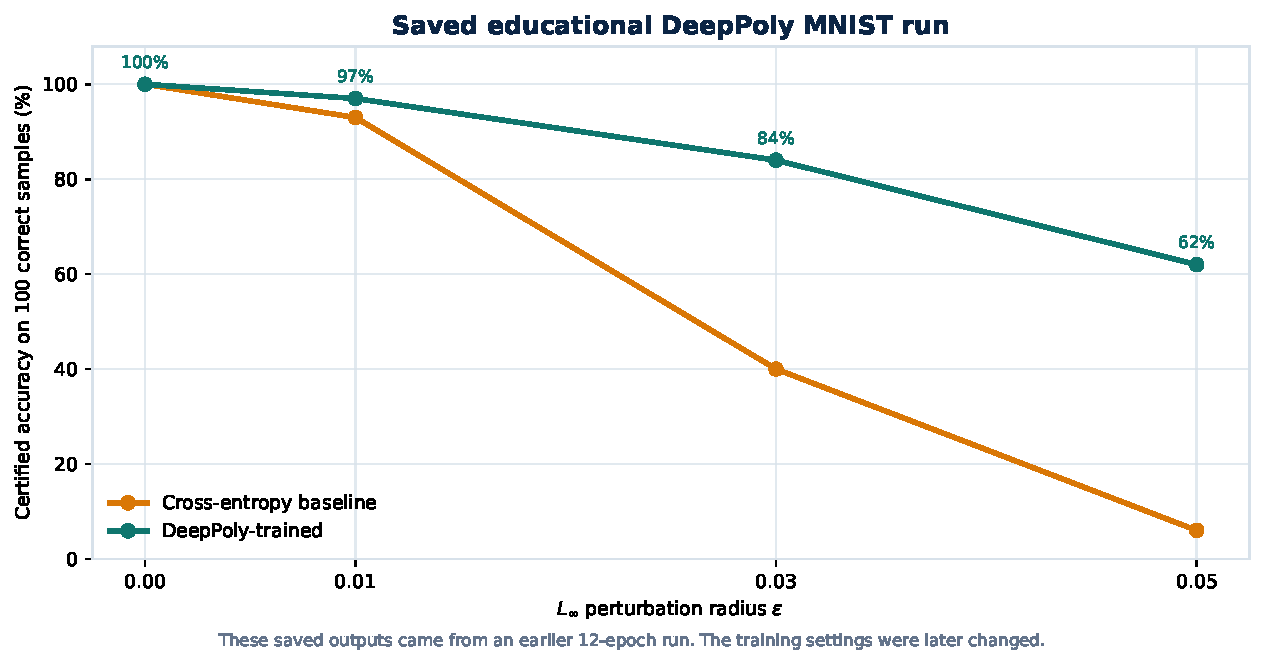
\includegraphics[width=0.76\textwidth]{sri_deeppoly_certification.pdf}
\caption{Certified accuracy from the saved educational MNIST experiment.}
\label{fig:deeppoly}
\end{figure}

\section{Study II: Proposed Zero-Knowledge Robustness Verification}

\subsection{Claim and trust boundary}

This study produced a system design, not an implementation. The intended public claim is that a stated number of committed evaluation samples satisfies a chosen robustness condition for a committed model. A complete relation would need to bind all components listed in Table~\ref{tab:zk-relation}.

\begin{table}[H]
\centering
\small
\caption{Proposed zero-knowledge relation for robustness verification.}
\label{tab:zk-relation}
\begin{tabularx}{\textwidth}{L{0.20\textwidth}Y}
\toprule
\textbf{Component} & \textbf{Proposed contents} \\
\midrule
Public inputs &
Model and dataset commitments, architecture description, perturbation radius, quantization scale, certification rule, claimed certified count, and proof-system parameters. \\
\addlinespace
Private witness &
Model weights, selected inputs and labels, intermediate affine values, activation-phase data, lower and upper bounds, and commitment openings. \\
\addlinespace
Circuit checks &
Commitment consistency, affine propagation, ReLU case constraints, range constraints, perturbation bounds, fixed-point overflow rules, final class separation, and certified-count aggregation. \\
\addlinespace
Required guarantees &
Proof soundness, hiding and binding commitments, unambiguous arithmetic semantics, and consistency between certificate generation and verification. \\
\bottomrule
\end{tabularx}
\end{table}

\subsection{Proposed workflow}

\begin{figure}[H]
\centering
\fcolorbox{researchblue}{researchlight}{
\parbox{0.76\textwidth}{
\centering
\textbf{Committed private model and evaluation data}\\
The prover holds weights, samples, labels, and commitment openings.
}}

\vspace{0.14cm}
\(\Downarrow\)
\vspace{0.14cm}

\fcolorbox{researchteal}{researchlight}{
\parbox{0.76\textwidth}{
\centering
\textbf{DeepPoly bound generation}\\
Generate candidate affine bounds, ReLU cases, ranges, and final margins.
}}

\vspace{0.14cm}
\(\Downarrow\)
\vspace{0.14cm}

\fcolorbox{researchnavy}{researchlight}{
\parbox{0.76\textwidth}{
\centering
\textbf{Proposed zero-knowledge checker}\\
Verify the complete consistency chain under fixed arithmetic semantics.
}}

\vspace{0.14cm}
\(\Downarrow\)
\vspace{0.14cm}

\fcolorbox{researchteal}{researchlight}{
\parbox{0.76\textwidth}{
\centering
\textbf{Public output}\\
Verify or reject the committed certified-count claim.
}}
\caption{Proposed private robustness-verification workflow. No circuit or proof was implemented.}
\label{fig:zk}
\end{figure}

Generating candidate bounds outside the circuit can reduce proof cost, but the circuit must still verify every consistency condition required by the public claim. Accepting unverified intermediate bounds would only prove that a submitted certificate has a desired final margin, not that it belongs to the committed model and data.

The unresolved engineering work includes quantization-error bounds, signed comparisons, ReLU phase encoding, memory requirements, batched certification, commitment design, and end-to-end proof benchmarking. These requirements make the proposal a separate research program rather than an empirical result of the internship.

\section{Study III: Frozen Cross-Victim RL Attack Transfer}

\subsection{Transfer setting and threat model}

The transferred object is a sequential attack policy, not a precomputed adversarial image. The target returns class scores for each submitted image. The attacker receives the clean image and label but no gradients, parameters, intermediate activations, training data, or architecture metadata.

The final study evaluates frozen transfer. Recurrent hidden state may change within one attack episode, but policy weights, optimizer state, observation normalization, and configuration remain unchanged after source training. A SHA-256 digest is checked before and after target evaluation. Target adaptation exists as a cloned-policy software path but was not evaluated in the final study.

The target protocol uses CIFAR-10 \cite{krizhevsky2009cifar}, an untargeted \(L_\infty\) bound of \(8/255\), and 25 total score calls including initialization. Attack success is measured only over images classified correctly before the attack. Every method uses the same eligible sample identities and derives all query checkpoints from one trajectory.

\begin{figure}[H]
\centering
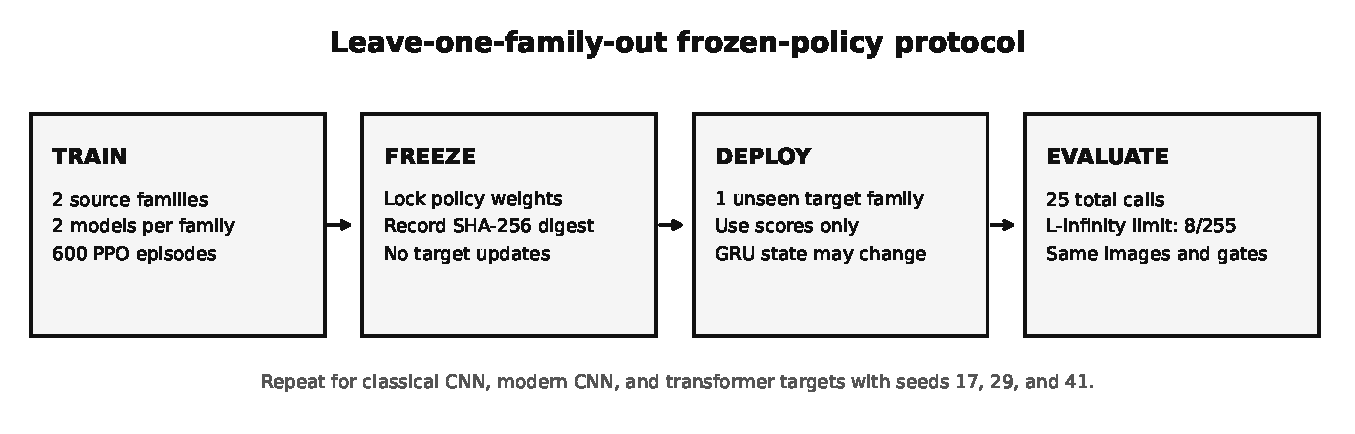
\includegraphics[width=\textwidth]{sri_rl_protocol.pdf}
\caption{Train, freeze, deploy, and evaluate protocol used in each family and seed fold.}
\label{fig:protocol}
\end{figure}

\subsection{Victim population and data}

Three custom CIFAR-scale victim families were used: a residual classical CNN with 2,777,674 parameters, a depthwise modern CNN with 1,223,738 parameters, and a patch transformer with 347,722 parameters. These are custom research models, not standard pretrained ResNet, ConvNeXt, or ViT checkpoints.

Each victim was trained on 10,000 CIFAR-10 images for 12 epochs. For each held-out family and seed, source training used two independently initialized instances from each of the other two families. One independently trained target instance represented the held-out family. Seeds 17, 29, and 41 produced nine separately trained policies and nine frozen evaluations. The data split included 1,000 policy-training images, 1,000 source-validation images, and 300 candidate target-test images per fold.

\begin{figure}[H]
\centering
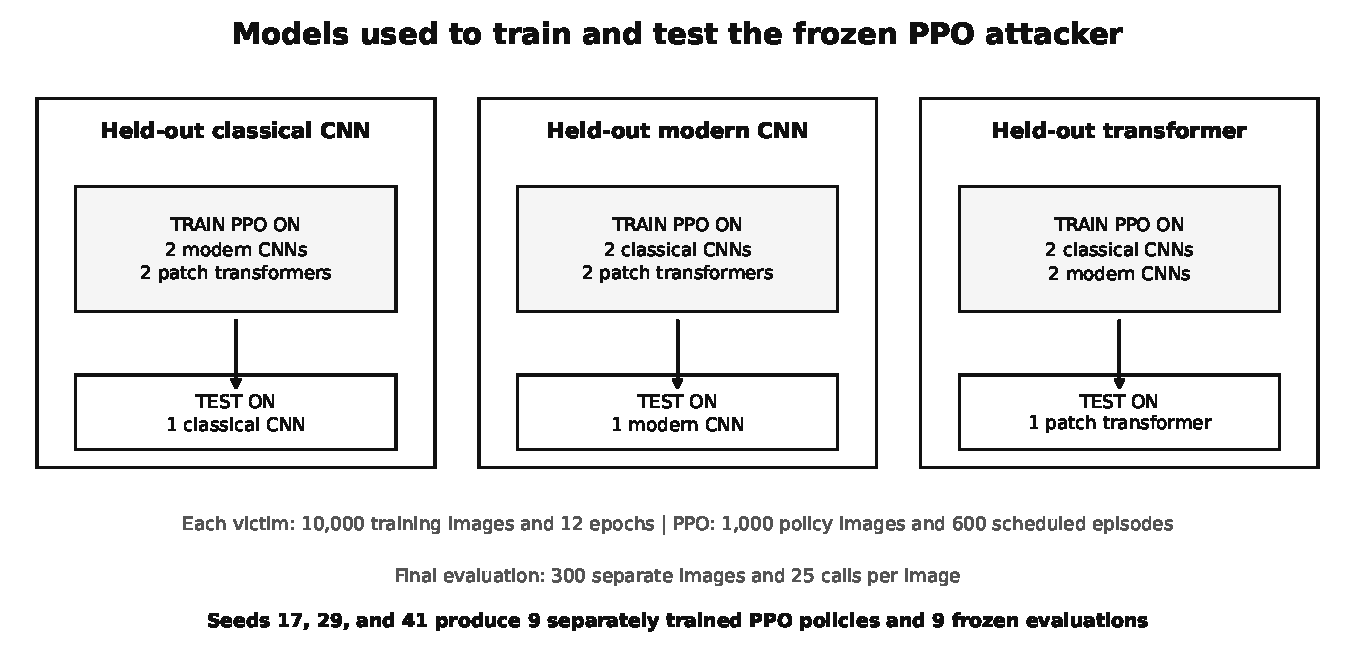
\includegraphics[width=\textwidth]{sri_rl_train_test_design.pdf}
\caption{Source and target arrangement for the leave-one-family-out study.}
\label{fig:train-test}
\end{figure}

\subsection{Policy, observation, and actions}

The recurrent actor-critic receives eight features: normalized true-class rank, predictive entropy, true-class score change, true-versus-rival margin, remaining-query fraction, previous-action identifier, transformed previous reward, and episode progress. A tanh encoder maps the observation to 96 dimensions. A 96-unit GRU supplies within-episode memory, followed by a 96-logit actor and a scalar critic.

\begin{figure}[H]
\centering
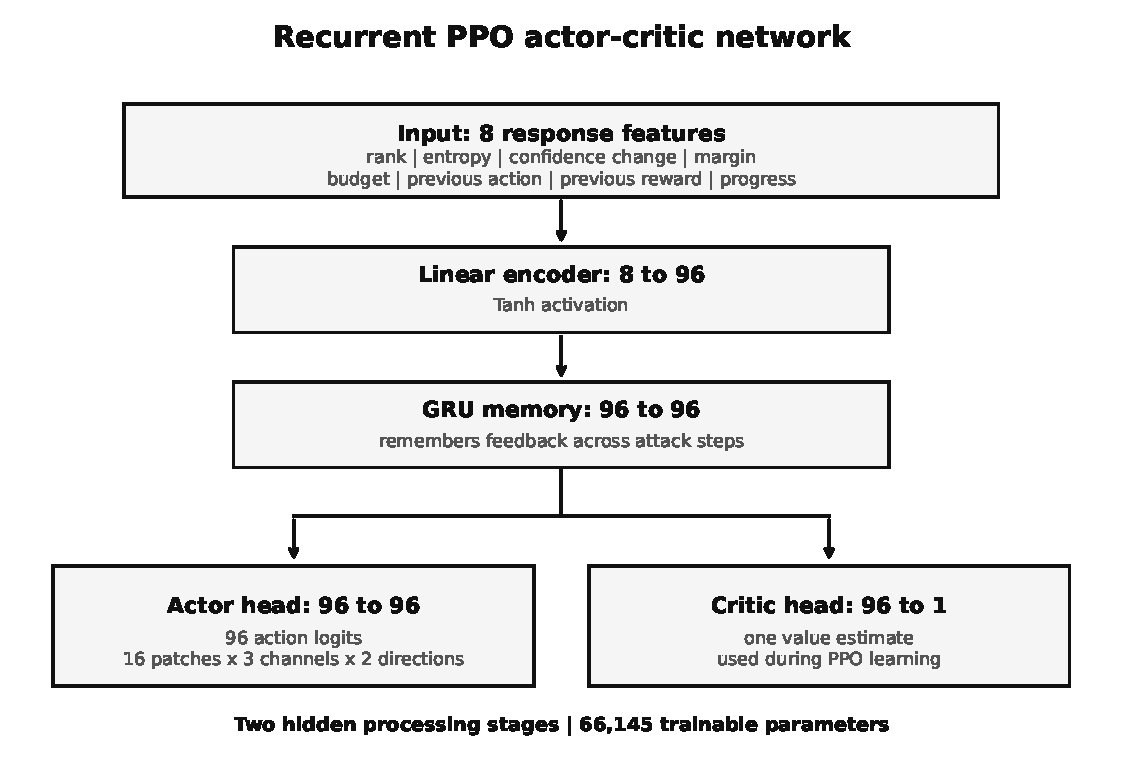
\includegraphics[width=0.88\textwidth]{sri_rl_policy_architecture.pdf}
\caption{Recurrent PPO actor-critic with 66,145 trainable parameters.}
\label{fig:policy}
\end{figure}

\begin{samepage}
The \(32\times32\) image is divided into a \(4\times4\) patch grid. An action selects one of 16 patches, one of three channels, and one sign, giving

\begin{equation}
|\mathcal{A}|=16\times3\times2=96.
\end{equation}

PPO changes the selected channel-patch region by \(2/255\). Each update is projected into the raw-pixel perturbation ball:

\begin{equation}
x_{t+1}
=
\operatorname{clip}_{[0,1]}
\left(
\operatorname{clip}_{[x-\varepsilon,x+\varepsilon]}
\left(x_t+\delta(a_t)\right)
\right).
\label{eq:projection}
\end{equation}
\end{samepage}

\subsection{Reward, optimization, and source balance}

Let

\begin{equation}
m_t=p_y(x_t)-\max_{j\neq y}p_j(x_t)
\end{equation}

be the true-class margin after query \(t\). The dense reward is

\begin{equation}
r_t
=
5(m_{t-1}-m_t)
+
2\,\mathbb{I}[f(x_t)\neq y]
-
0.01.
\label{eq:reward}
\end{equation}

PPO uses learning rate \(3\times10^{-4}\), clip ratio \(0.2\), value-loss coefficient \(0.5\), entropy coefficient \(0.01\), gradient-norm limit \(0.5\), four optimization epochs per collection block, and discount \(0.98\). Source families are scheduled in balanced cycles. GroupDRO weights increase for families with worse episodic return.

Each run schedules 600 policy episodes and updates after blocks of 25. Across nine runs, 5,400 episodes were scheduled, but only 3,640 produced clean-correct trainable sequences. The other episodes were ineligible because the assigned source victim already misclassified the clean image.

\subsection{Controls, metrics, and promotion rule}

The primary controls are uniform random actions, an episode-local score bandit, and score-greedy patch search. Score greedy uses the same images, patch-direction catalog, final perturbation bound, and total target-call budget. It differs in two important ways: it proposes a direct \(8/255\) change rather than PPO's \(2/255\) step, and it retains a proposal only when the margin improves. It is therefore a strong query-driven control, but not an action-operator-matched comparison.

For a set of clean-correct target outcomes,

\begin{equation}
\operatorname{ASR}(q)
=
\frac{
\text{successful attacks by total call }q
}{
\text{clean-correct eligible cases}
}.
\end{equation}

ASR is recorded at total call budgets \(0,5,10,\) and \(25\). Query efficiency is summarized by a normalized trapezoidal area,

\begin{equation}
\operatorname{AUC}
=
\frac{1}{q_K-q_0}
\sum_{k=0}^{K-1}
(q_{k+1}-q_k)
\frac{\operatorname{ASR}(q_k)+\operatorname{ASR}(q_{k+1})}{2}.
\label{eq:auc}
\end{equation}

The promotion rule requires a complete family and seed grid, passing victim gates, three seeds per family, positive paired Student-\(t\) 95\% lower bounds for PPO minus every control in both final ASR and AUC, mean gains of at least 0.01 ASR and 0.005 AUC, and normalized executed-action entropy in \([0.10,0.95]\) for every seed.

\subsection{Compute and reproducibility}

The final study ran on Apple M4 MPS with macOS 15.7.3 arm64, Python 3.13.11, PyTorch 2.13.0, and torchvision 0.28.0. It recorded 91,800 source-model calls and completed in 6,864.9 seconds, or 114.4 minutes. PyTorch warned that one MPS operation lacked a deterministic implementation, so checkpoint and result digests are used alongside seeds.

\section{Results}

\subsection{Victim quality}

All configured victim gates passed. The gate thresholds were \(60\%\) for the classical CNN, \(50\%\) for the modern CNN, and \(40\%\) for the transformer.

\begin{figure}[H]
\centering
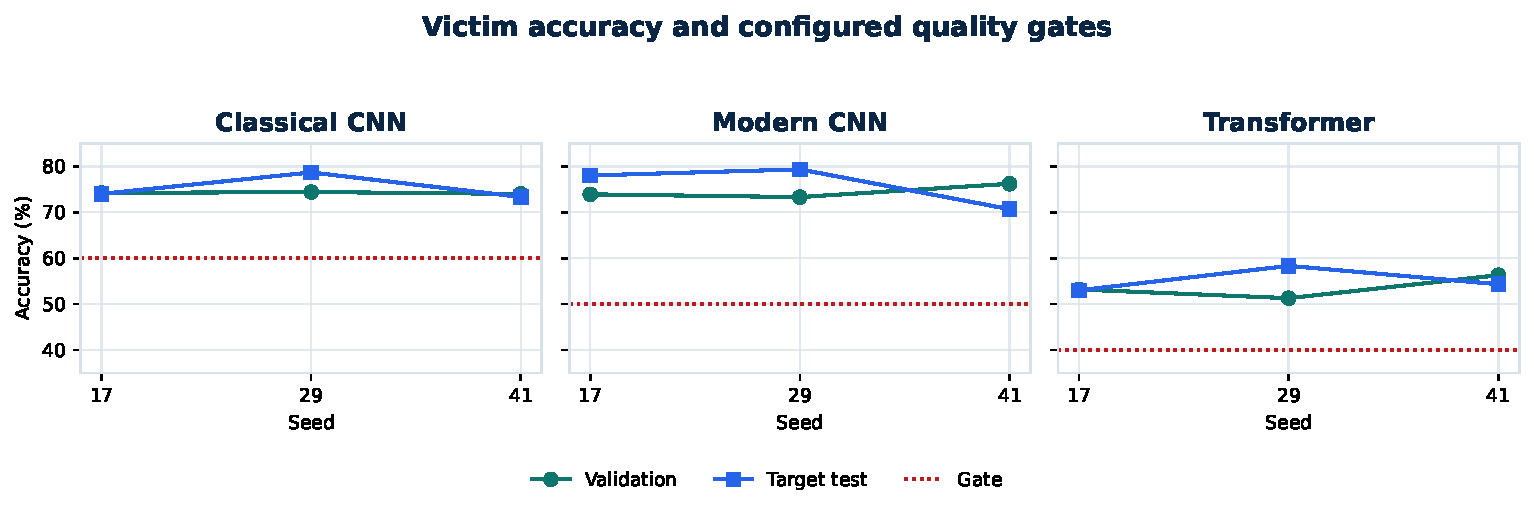
\includegraphics[width=\textwidth]{sri_victim_accuracy.pdf}
\caption{Validation and target-test accuracy for the nine held-out victim runs.}
\label{fig:victim}
\end{figure}

\begin{table}[H]
\centering
\caption{Victim accuracy ranges across the three target seeds.}
\begin{tabularx}{0.92\textwidth}{Y C{0.22\textwidth} C{0.16\textwidth} C{0.22\textwidth}}
\toprule
\textbf{Family} & \textbf{Validation} & \textbf{Gate} & \textbf{Target test} \\
\midrule
Classical CNN & \(74.0\%\) to \(74.4\%\) & \(60\%\) & \(73.3\%\) to \(78.7\%\) \\
Modern CNN & \(73.3\%\) to \(76.2\%\) & \(50\%\) & \(70.7\%\) to \(79.3\%\) \\
Transformer & \(51.3\%\) to \(56.3\%\) & \(40\%\) & \(53.0\%\) to \(58.3\%\) \\
\bottomrule
\end{tabularx}
\end{table}

The transformer is weaker than the two CNN families, which limits cross-family comparison and external validity. It nevertheless exceeded its prespecified gate in every seed.

\subsection{Final attack success}

\begin{figure}[H]
\centering
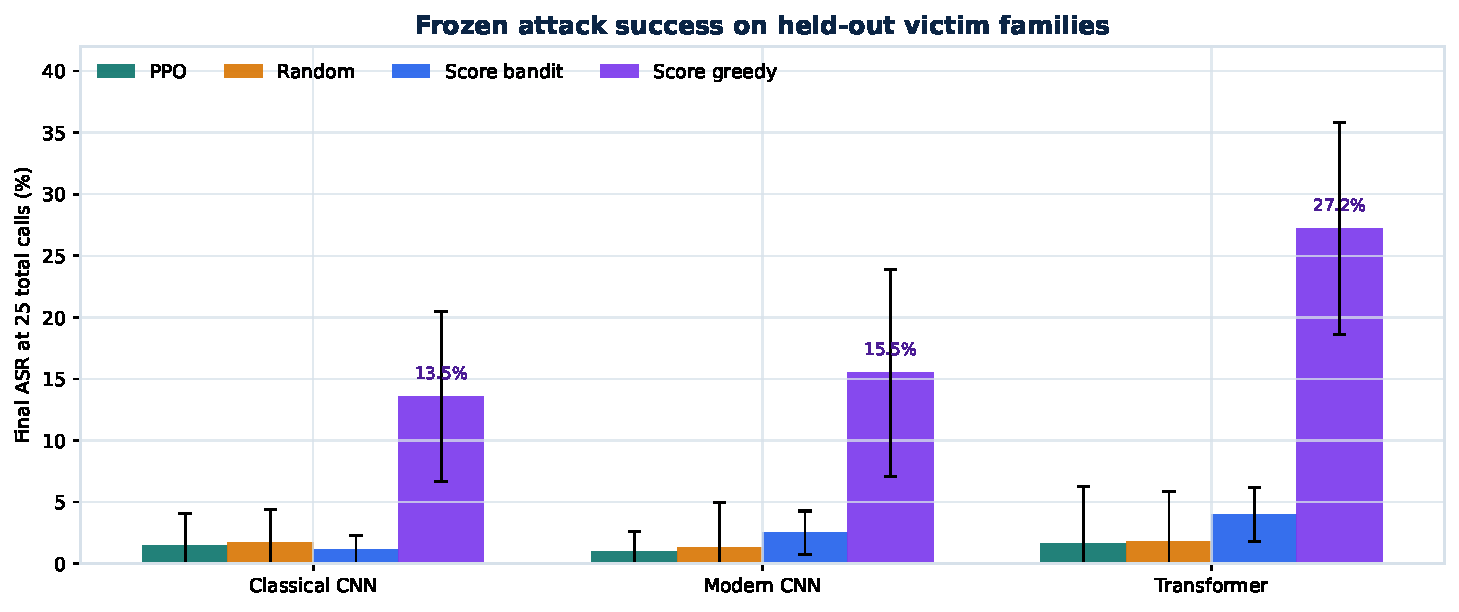
\includegraphics[width=\textwidth]{sri_final_asr.pdf}
\caption{Mean final attack success at 25 total target calls.}
\label{fig:asr}
\end{figure}

\begin{table}[H]
\centering
\small
\caption{Final ASR in percent, reported as mean [Student-\(t\) 95\% interval] over three seeds.}
\label{tab:asr}
\setlength{\tabcolsep}{3.5pt}
\begin{tabularx}{\textwidth}{Y C{0.175\textwidth} C{0.175\textwidth} C{0.175\textwidth} C{0.175\textwidth}}
\toprule
\textbf{Held-out family} & \textbf{PPO} & \textbf{Random} & \textbf{Bandit} & \textbf{Score greedy} \\
\midrule
Classical CNN &
\shortstack{1.45\\\mbox{[0.00, 4.05]}} &
\shortstack{1.74\\\mbox{[0.00, 4.43]}} &
\shortstack{1.17\\\mbox{[0.04, 2.30]}} &
\shortstack{13.55\\\mbox{[6.65, 20.45]}} \\
Modern CNN &
\shortstack{1.01\\\mbox{[0.00, 2.59]}} &
\shortstack{1.29\\\mbox{[0.00, 4.95]}} &
\shortstack{2.50\\\mbox{[0.72, 4.28]}} &
\shortstack{15.49\\\mbox{[7.05, 23.92]}} \\
Transformer &
\shortstack{1.65\\\mbox{[0.00, 6.29]}} &
\shortstack{1.84\\\mbox{[0.00, 5.90]}} &
\shortstack{4.02\\\mbox{[1.83, 6.21]}} &
\shortstack{27.20\\\mbox{[18.61, 35.79]}} \\
\bottomrule
\end{tabularx}
\end{table}

PPO did not exceed random on any family mean. Pooled descriptively across the nine runs, PPO succeeded on 25 of 1,859 eligible cases, random on 30, score bandit on 45, and score greedy on 333. The family-level, equal-seed summaries remain primary because pooled counts give different weights to runs with different eligible sample counts.

\subsection{Query efficiency}

\begin{figure}[H]
\centering
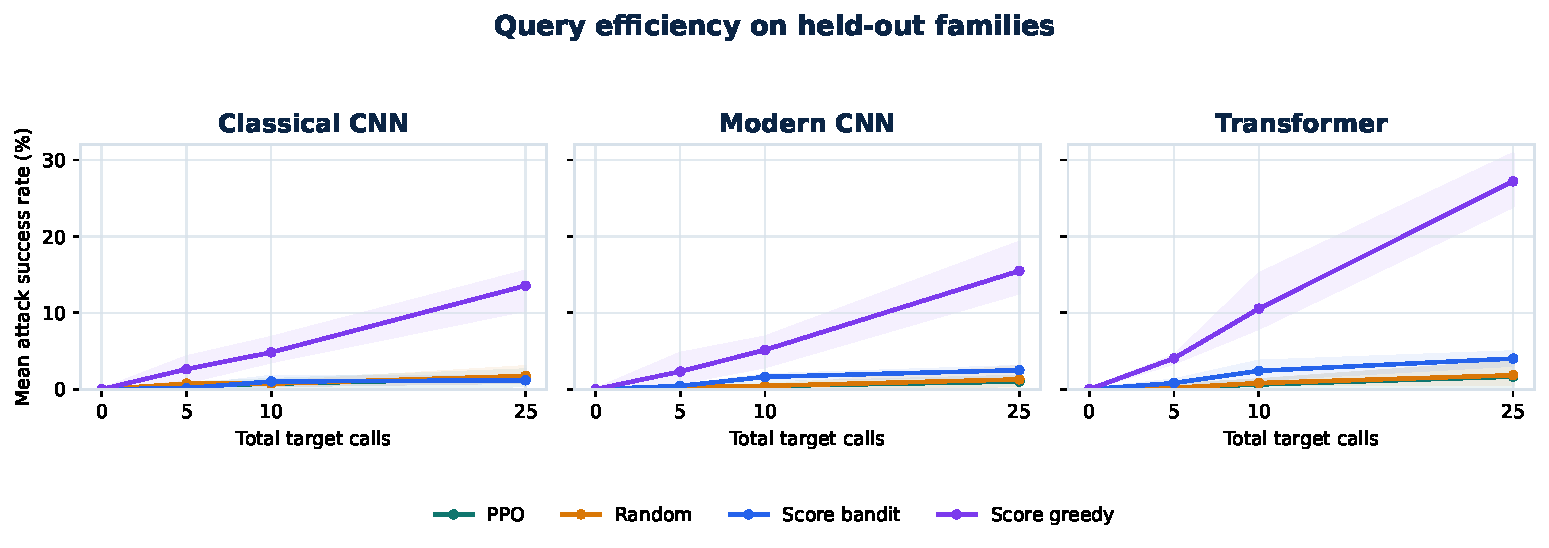
\includegraphics[width=\textwidth]{sri_query_curves.pdf}
\caption{Across-seed ASR as the total target-call budget is consumed.}
\label{fig:query}
\end{figure}

\begin{table}[H]
\centering
\caption{Mean normalized ASR-query AUC in percentage points.}
\setlength{\tabcolsep}{4pt}
\begin{tabularx}{0.92\textwidth}{Y C{0.15\textwidth} C{0.15\textwidth} C{0.15\textwidth} C{0.15\textwidth}}
\toprule
\textbf{Held-out family} & \textbf{PPO} & \textbf{Random} & \textbf{Bandit} & \textbf{Score greedy} \\
\midrule
Classical CNN & 0.81 & 0.96 & 0.79 & 6.52 \\
Modern CNN & 0.53 & 0.62 & 1.48 & 7.17 \\
Transformer & 0.78 & 0.91 & 2.33 & 13.19 \\
\bottomrule
\end{tabularx}
\end{table}

PPO remained close to random across the complete query trajectory. Its low final ASR cannot be explained by a delayed advantage appearing only near query 25.

\subsection{Executed-action entropy and source diagnostics}

\begin{figure}[H]
\centering
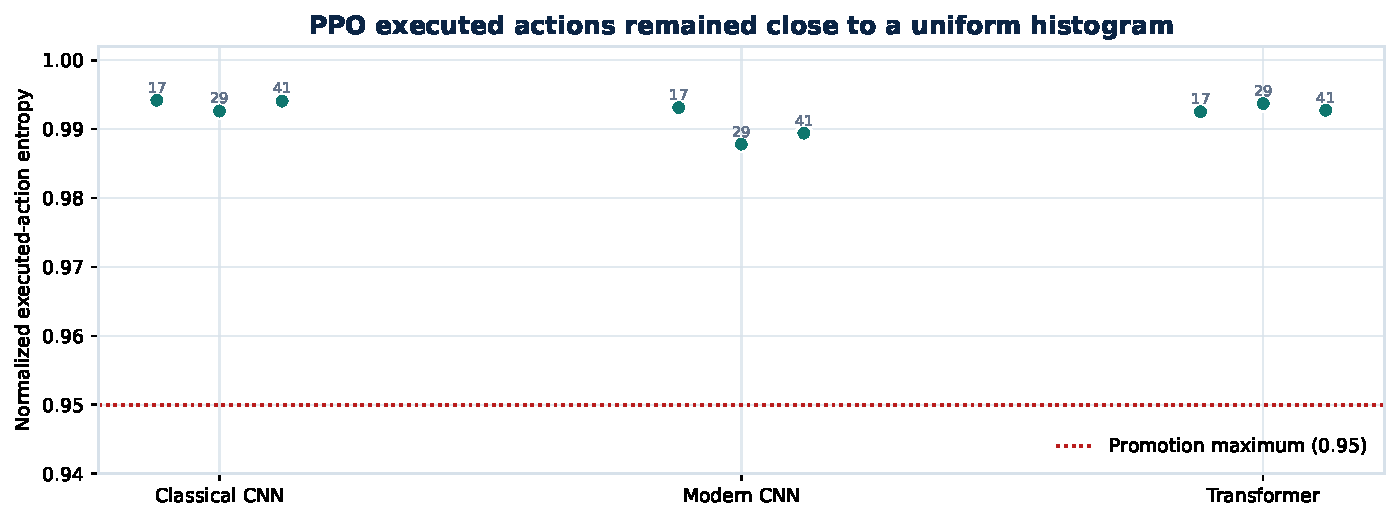
\includegraphics[width=0.88\textwidth]{sri_action_entropy.pdf}
\caption{Normalized entropy of executed PPO actions. The promotion ceiling is 0.95.}
\label{fig:entropy}
\end{figure}

Executed-action entropy ranged from 0.988 to 0.994 across the nine runs, above the promotion ceiling in every seed. This is the entropy of the aggregate executed-action histogram. It does not prove that every state-conditioned actor distribution was uniform.

Only 64 of 3,640 trainable source episodes ended in attack success, a rate of \(1.76\%\). Combined with the near-uniform target action histogram, this motivates a weak source-learning hypothesis. The target-only experiment cannot distinguish weak source competence from a separate loss of transfer during deployment.

\subsection{Promotion outcome}

\finding{Measured outcome.}{All three held-out families failed the promotion rule. The run grid was complete, all victim gates passed, target policies remained frozen, eligible cohorts and query checkpoints aligned, and the result manifest passed internal recomputation. The failure was caused by ASR, AUC, and entropy values rather than invalid or missing runs.}

\section{Discussion}

\subsection{Interpretation of the RL result}

The tested PPO configuration did not establish a frozen cross-victim advantage. PPO final ASR and query AUC were close to random, and aggregate executed actions remained near a uniform histogram. This conclusion is limited to the implemented observation, action catalog, reward, training schedule, source population, and query budget.

Score-greedy search achieved higher ASR in every held-out family. That result establishes that query-driven patch search can exploit the target scores under the overall threat setting. It does not establish that PPO failed under an identical operator because greedy used \(8/255\) proposals, kept only improvements, and therefore combined action magnitude, selection, and rollback advantages.

\subsection{Competing explanations}

Two explanations remain unresolved. First, the source task may not have been learned well enough. Only \(1.76\%\) of trainable source episodes ended in success, and no complete source-versus-held-out competence curve was recorded for the final policy. Second, the policy may have learned source-specific behavior that failed to generalize across families. Source-model, new-instance, and held-out-family evaluations are required to separate these cases.

The eight-dimensional observation also omits image content, patch visit counts, perturbation state by region, and an explicit accepted-action history. Distinct attack situations can therefore map to similar observations. The GRU can preserve received information, but it cannot recover information absent from the observation.

\subsection{Relationship among the three studies}

The three work packages address different guarantees. DeepPoly asks whether every permitted input in a local region preserves the prediction. The proposed zero-knowledge relation asks whether that certification computation can be checked without revealing its witness. The RL study asks whether limited target scores support a reusable attack policy. No combined DeepPoly and zero-knowledge system, or DeepPoly-certified defense against the RL attacker, was evaluated.

\subsection{Limitations}

\begin{itemize}
  \item The DeepPoly result uses a saved 100-sample educational run and ambiguous cohort metadata.
  \item The DeepPoly implementation was not independently audited for numerical soundness.
  \item The zero-knowledge component is a design proposal with no circuit, proof, or performance data.
  \item The RL study uses CIFAR-10, three seeds, custom compact victims, and one held-out target instance per family and seed.
  \item The transformer family has lower clean accuracy than the CNN families.
  \item PPO and score greedy differ in step size and rollback behavior.
  \item The 25-call budget is narrow, and established Square Attack, SimBA-DCT, NES, and HopSkipJump implementations were not included.
  \item Target adaptation and sequential retention were not evaluated, so the results do not establish continual learning.
  \item Student-\(t\) intervals over three seeds are descriptive and wide.
  \item One MPS operation is not fully deterministic.
\end{itemize}

These limitations prevent general claims about RL attacks, architecture-family transfer, production transformers, or private robustness verification.

\section{Prioritized Future Experiments}

\begin{enumerate}
  \item \textbf{Measure source competence.}
  Evaluate each checkpoint on the exact source instances, new instances from seen families, and the held-out family. Do not proceed to a transfer claim until the policy beats matched random search on source validation.

  \item \textbf{Match the action operator.}
  Compare \(2/255\), \(4/255\), and \(8/255\) proposals under the same accept-or-reject rule for PPO, random, bandit, and greedy methods.

  \item \textbf{Initialize from demonstrations.}
  Collect successful score-greedy trajectories on source victims, train the actor by behavior cloning, and then fine-tune with PPO.

  \item \textbf{Add explicit state information.}
  Test patch visit counts, signed score changes, perturbation magnitude by region, recent accepted actions, and a compact patch embedding.

  \item \textbf{Factor the action space.}
  Use hierarchical decisions for region, channel, sign, and step size. Compare coarse and fine patch grids under matched budgets.

  \item \textbf{Increase source diversity only after a learning gate passes.}
  Add independently trained victim instances and standard architecture families, then repeat at least three seeds.

  \item \textbf{Evaluate target adaptation separately.}
  Clone the source policy, update only the clone on a disjoint adaptation split, and evaluate on untouched target data. Measure retention before using the term continual learning.

  \item \textbf{Implement a minimal zero-knowledge checker.}
  Begin with one affine layer and one ReLU under fixed-point arithmetic. Bind all values to commitments, test overflow constraints, and compare proof cost with direct public verification.
\end{enumerate}

\section{Responsible Use and Reproducibility}

The attack code is intended for authorized defensive robustness research on public benchmarks or systems the researcher owns or has explicit permission to test. Query limits, service terms, and disclosure requirements must be respected. Pretrained transferable attack policies require additional dual-use review before public release.

The final RL configuration is stored in
\path{configs/rl_transfer/cifar10_m4_study.json}, with per-run settings in
\path{configs/rl_transfer/cifar10_m4_iteration.json}. Verified compact results are in
\path{docs/research/cifar10_m4_study_results.json}. The notebook
\path{notebooks/cifar10_m4_study.ipynb} provides interactive analysis, and
\path{MODEL_CARD_RL_ATTACK.md} records the responsible-use boundary. The final study code revision is
\texttt{2eb481a}. The public repository is
\url{https://github.com/jeetrex17/deeppoly}.

\section{Conclusion}

The strongest measured result is negative: across nine frozen target evaluations, the tested recurrent GroupDRO PPO policy remained close to random and failed the prespecified promotion rule, while score-greedy patch search achieved higher ASR. The protocol itself completed as intended, with passing victim gates, stable policy digests, matched cohorts, and consistent query accounting.

The DeepPoly stage demonstrated certification-aware training in a saved educational MNIST run, but the result is tied to an early configuration and does not constitute a benchmark or independent verifier audit. The zero-knowledge stage identified the relation and constraints required for private robustness verification, but no circuit or proof was implemented.

The next empirical decision is therefore narrow: establish source-task competence under an operator-matched comparison before spending more compute on held-out transfer. Behavior cloning from successful greedy trajectories, richer state features, and controlled action ablations provide direct tests of the observed failure modes.

\section*{Acknowledgement}

We thank Prof. Manik Lal Das for mentoring this Summer Research Internship and DA-IICT for providing the academic setting for the work.

\clearpage
\appendix

\section{RL Hyperparameters}

\begin{table}[H]
\centering
\small
\caption{Core configuration of the final frozen-policy study.}
\begin{tabularx}{0.90\textwidth}{L{0.38\textwidth}Y}
\toprule
\textbf{Item} & \textbf{Value} \\
\midrule
Dataset & CIFAR-10 \\
Target families & Classical CNN, modern CNN, patch transformer \\
Seeds & 17, 29, 41 \\
Victim fitting & 10,000 images, 12 epochs, AdamW, cosine schedule \\
Policy data & 1,000 training images and 1,000 source-validation images \\
Policy schedule & 600 episodes per run, blocks of 25 \\
Policy architecture & 8-feature tanh encoder, 96-unit GRU, 96-action actor, scalar critic \\
PPO learning rate & \(3\times10^{-4}\) \\
PPO clip ratio & 0.2 \\
Value and entropy coefficients & 0.5 and 0.01 \\
PPO update epochs & 4 \\
Discount & 0.98 \\
Action step and bound & \(2/255\) step; \(8/255\) final \(L_\infty\) bound \\
Target budget & 25 total calls including initialization \\
\bottomrule
\end{tabularx}
\end{table}

\section{Per-Seed Final ASR}

\begin{table}[H]
\centering
\small
\caption{Final ASR in percent for each held-out family and seed.}
\setlength{\tabcolsep}{3.5pt}
\begin{tabularx}{\textwidth}{Y C{0.07\textwidth}C{0.09\textwidth}C{0.09\textwidth}C{0.09\textwidth}C{0.11\textwidth}C{0.08\textwidth}}
\toprule
\textbf{Family} & \textbf{Seed} & \textbf{PPO} & \textbf{Random} & \textbf{Bandit} & \textbf{Greedy} & \textbf{Eligible} \\
\midrule
Classical CNN & 17 & 1.35 & 1.35 & 0.90 & 10.36 & 222 \\
Classical CNN & 29 & 2.54 & 2.97 & 1.69 & 14.83 & 236 \\
Classical CNN & 41 & 0.45 & 0.91 & 0.91 & 15.45 & 220 \\
\addlinespace
Modern CNN & 17 & 1.71 & 2.99 & 2.99 & 19.23 & 234 \\
Modern CNN & 29 & 0.84 & 0.42 & 1.68 & 12.61 & 238 \\
Modern CNN & 41 & 0.47 & 0.47 & 2.83 & 14.62 & 212 \\
\addlinespace
Transformer & 17 & 1.26 & 1.26 & 3.14 & 30.82 & 159 \\
Transformer & 29 & 0.00 & 0.57 & 4.00 & 26.86 & 175 \\
Transformer & 41 & 3.68 & 3.68 & 4.91 & 23.93 & 163 \\
\bottomrule
\end{tabularx}
\end{table}

\section{Pilot Scope}

The preliminary Apple M4 pilot trained on classical and modern CNN sources and evaluated a held-out patch transformer. It completed in 6 minutes 12 seconds over 99 clean-correct target images. Stochastic PPO reached \(5.1\%\) final ASR and random reached \(7.1\%\). The pilot verified MPS execution and frozen-policy digest checks. Its training conditions differ from the final study, so it is not treated as a repeated measurement of the nine-run experiment.

\begin{thebibliography}{99}

\bibitem{szegedy2014intriguing}
C. Szegedy et al.,
``Intriguing properties of neural networks,''
International Conference on Learning Representations, 2014.

\bibitem{goodfellow2015explaining}
I. J. Goodfellow, J. Shlens, and C. Szegedy,
``Explaining and harnessing adversarial examples,''
International Conference on Learning Representations, 2015.

\bibitem{madry2018towards}
A. Madry, A. Makelov, L. Schmidt, D. Tsipras, and A. Vladu,
``Towards deep learning models resistant to adversarial attacks,''
International Conference on Learning Representations, 2018.

\bibitem{singh2019deeppoly}
G. Singh, T. Gehr, M. P{\"u}schel, and M. Vechev,
``An abstract domain for certifying neural networks,''
Proceedings of the ACM on Programming Languages, vol. 3, POPL, 2019.

\bibitem{schulman2017ppo}
J. Schulman, F. Wolski, P. Dhariwal, A. Radford, and O. Klimov,
``Proximal policy optimization algorithms,''
arXiv:1707.06347, 2017.

\bibitem{sagawa2020groupdro}
S. Sagawa, P. W. Koh, T. B. Hashimoto, and P. Liang,
``Distributionally robust neural networks for group shifts,''
International Conference on Learning Representations, 2020.

\bibitem{guo2019simba}
C. Guo, J. R. Gardner, Y. You, A. G. Wilson, and K. Q. Weinberger,
``Simple black-box adversarial attacks,''
International Conference on Machine Learning, 2019.

\bibitem{liu2021zkcnn}
T. Liu, X. Xie, and Y. Zhang,
``zkCNN: Zero knowledge proofs for convolutional neural network predictions and accuracy,''
ACM SIGSAC Conference on Computer and Communications Security, 2021.

\bibitem{feng2021zen}
B. Feng et al.,
``ZEN: An optimizing compiler for verifiable, zero-knowledge neural network inferences,''
Cryptology ePrint Archive, Report 2021/087, 2021.

\bibitem{kothapalli2022nova}
A. Kothapalli, S. Setty, and I. Tzialla,
``Nova: Recursive zero-knowledge arguments from folding schemes,''
Annual International Cryptology Conference, 2022.

\bibitem{bunz2018bulletproofs}
B. B{\"u}nz, J. Bootle, D. Boneh, A. Poelstra, P. Wuille, and G. Maxwell,
``Bulletproofs: Short proofs for confidential transactions and more,''
IEEE Symposium on Security and Privacy, 2018.

\bibitem{krizhevsky2009cifar}
A. Krizhevsky,
``Learning multiple layers of features from tiny images,''
Technical report, University of Toronto, 2009.

\end{thebibliography}

\end{document}
